\documentclass[10pt,a4paper]{report}
\usepackage[utf8]{inputenc}
\usepackage[english]{babel}
\usepackage{amsmath}
\usepackage{amsfonts}
\usepackage{amssymb}
\usepackage{wrapfig}
\usepackage{graphicx}
\graphicspath{{./Images/}}
\usepackage{listings}
\usepackage{color}

\definecolor{dkgreen}{rgb}{0,0.6,0}
\definecolor{gray}{rgb}{0.5,0.5,0.5}
\definecolor{mauve}{rgb}{0.58,0,0.82}

\lstset{frame=tb,
  language=Python,
  aboveskip=3mm,
  belowskip=3mm,
  showstringspaces=false,
  columns=flexible,
  basicstyle={\small\ttfamily},
  numbers=none,
  numberstyle=\tiny\color{gray},
  keywordstyle=\color{blue},
  commentstyle=\color{dkgreen},
  stringstyle=\color{mauve},
  breaklines=true,
  breakatwhitespace=true,
  tabsize=3
}
\pagenumbering{roman}

\title{Using Keystroke Dynamics to Authenticate a User Based on their Typing}
\author{Jack Francis}
\date{\today}

\begin{document}

\maketitle

\begin{abstract}
Hello
\end{abstract}

\tableofcontents

\pagenumbering{arabic}

\chapter{Introduction}
\setcounter{page}{1}

\chapter{Survey of Literature}

\chapter{Design and Implementation}

The following procedure from section 3.2 onwards is a rough implementation of the validation procedure by Ramin Toosi and Mohammad Ali Akhaee in their excellent paper 'Time–frequency analysis of keystroke dynamics for user authentication'. \cite{ToosiRamin2021Taok} The paper is theoretical in nature and describes an approach for performing validation on one word and then comparing them. It is in essence a one-time system whilst mine is a continuous system that aims to keep the user safe. In my project I've modified and implemented their validation approach whilst adding data gathering, word forming, word selection, word storage and update function. 

\section{Data gathering and Forming}
My program relies on capturing the users keystrokes and then processing them and then comparing them using a similarity measure. In order to do this, I decided to use the Keyboard Library REFERENCE HERE as it is a lightweight, secure and modern library that makes capturing keystrokes easy. In my project, I make use of the hook function of the library which is used to "hook" onto a users keyboard and record all of the users actions in and create keyboard events for each action. The record function which makes use of this hook function is shown in figure \ref{fig:Record}. The code snippet is very simple, first the program will 'hook' onto the keyboard using the Keyboard Libary mentioned above, record all keystrokes until the interval has passed and then stop recording. The start time of the interval and an array of Keyboard Events are then returned to the main body of the program. The start time of the interval is recorded and returned as it used further on in order to be able to place keyboard events on a time line in the context of the interval.

\begin{figure}[h!]
	\begin{lstlisting}
		def record(interval):
    		recorded = []
    		startTime = time.time()
    		keyBoardHook = keyboard.hook(recorded.append)
    		time.sleep(interval)
    		keyboard.unhook(keyBoardHook)
    		return recorded, startTime
	\end{lstlisting}
	\caption{Record Function}
	\label{fig:Record}
\end{figure}

A keyboard event is generated every time the user does something on the keyboard, whether that be pressing or releasing a key. Further information such as the type of the action (whether it was an a press or a release), which key is this action happening on and a a highly accurate time stamp of when the event occurred. Figure \ref{fig:Hook}, shows an example of a keyboard event produced by the function when the user presses down the 'h' key.

\begin{figure}[h]
\centering
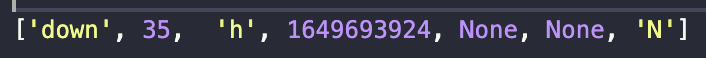
\includegraphics[scale=0.97]{KeyboardEvent}
\caption{The keyboard representation of a user pressing "h"}
\label{fig:Hook}
\end{figure}

The first element in the array is the action, this can be either 'up' or 'down' which are both self-explanatory. The next field is the scan-code which is a field I don't use but is useful for identifying keys easily. After this, is the name of the key which in this case is 'h' as we pressed the 'h' key down. The next field is the time since the epoch in seconds which is useful as it is this precise time-stamp that is used to do the rest of the calculations. The other three fields are device, modifiers and whether or not the user used a keypad. None of these I use in my program and as such are discarded almost immediately.

A small amount of pre-processing is then done on this data before it is paired up. The first step is to remove the scan code, keypad, modifier and device from each keyboard event and convert them into something lighter and more usable. The next step is to take the start time that is returned by the record function and subtract this from the time stamp in each keyboard event to get the time that the action occurred in the interval. Figure \ref{fig:preproc} shows what the data in \ref{fig:Hook} looks like after going through this.

\begin{wrapfigure}{l}{0.5\textwidth}
	\begin{center}
		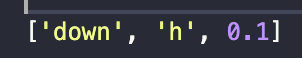
\includegraphics[width=0.48\textwidth]{KeyboardEventPreProc}
	\end{center}
	\caption{Keyboard representation of a user pressing 'h' after pre-processing}
	\label{fig:preproc}
\end{wrapfigure}

The data collected at this point is stored as a 2D array with each sub array corresponding to an action. An example sub array is shown in \ref{fig:preproc}.

In this form the data is unable to be used for anything, as it currently takes the form of a number of individual actions seem to have no relation to one another. Therefore, the next step is to form pairs from the data. A pair is formed of when 'down' action and one 'up' action where the key field matches and the 'down' is before the 'up'. The reason this is done is that it allows the program to work half as much data which reduces the number of unnecessary data points and allow the program to be able to form words using these pairs.

\begin{wrapfigure}{r}{0.4\textwidth}
	\begin{center}
		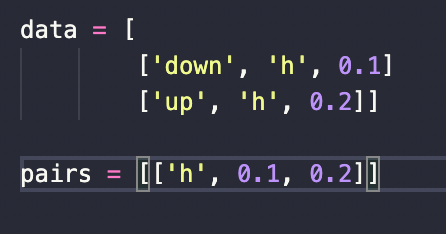
\includegraphics[width=0.38\textwidth]{SimplePairing}
	\end{center}
	\caption{Example of simple pairing}
	\label{fig:SimpPair}
\end{wrapfigure}

There are two main rules to follow when pairing the data. Due to the nature of how the data is collected, it is currently stored in chronological order which is very useful. In many cases, the user will press and release a key in quick succession without pressing any other keys. Due to the chronological nature of the data, pairing theses types of presses is easy. All that is needs to be done is to iterate through the pairs and when we come to a 'down' action then simply select the next value in the array if it is an 'up' action and the key matches. Figure \ref{fig:SimpPair} shows an example of this type or pairing. However, this type of nice easy matching is not always the case.

In some cases, a user may press more than one key down at once. This might occur when the user is capitalising words using 'shift' or when the user is typing fast so they may be already pressing down the next key before releasing the previous. An example of what the data will look like when this is the case is shown in Figure \ref{fig:WrongPair}. Applying the previous method in which we pair up keys with matching key types and opposite actions which are next to each other would result in the output shown in the pairs array. As you can see, this is not correct and would only lead to one pair where there should be two.

\begin{wrapfigure}{r}{0.4\textwidth}
	\begin{center}
		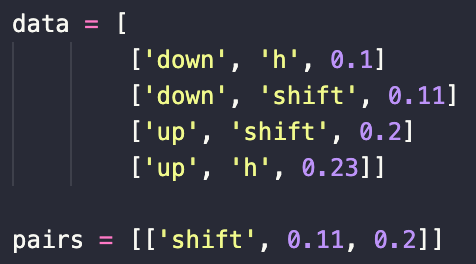
\includegraphics[width=0.38\textwidth]{PairingWrong}
	\end{center}
	\caption{Example of simple pairing}
	\label{fig:WrongPair}
\end{wrapfigure}

In order to fix this, it is necessary to include another case in the code. If the current action doesn't have a matching key and opposite action next in the array, then the program will iterate through the rest of the array starting from the current point in it searching for the next entry with a matching key and an opposite action that is after the current. If it finds one it will then pair them up. The key thing we assume for this to work is that every action has an opposite action. In nearly all cases we assume this to be true as it is highly unlikely that a user will hold down a key for the entire interval. If in a rare case this occurs however, this is handled. If the method cannot find a pair, then it is still added to the pairs list with an end time of the length of the interval.

The finished algorithm is shown in Figure \ref{fig:PairForm}. The reason for the error handling is that when coming to the end of the data, attempting to access the next element to check if it can be paired up results in an index error.
\begin{figure}[h!]
	\begin{lstlisting}
		def rawPairs(self):
        """
        Converts the array from the process function into key pairs

        Returns:
            2D array: Consisting of a pair of actions from the array above.
        """
        pairsArray = []
        for i in range(len(self.processed)):
            try:
                
                if (self.processed[i][2] == 'down' and self.processed[i+1][2] == 'up' and self.processed[i][0].lower() == self.processed[i+1][0].lower()):
                    # If the next value in the array is the up action
                    pairsArray.append([self.processed[i][0], self.processed[i][1], self.processed[i+1][1]])
                else:
                    # Otherwise, search for the next opposing action and pair them up
                    for x in range(i, len(self.processed)):
                        if (self.processed[x][0].lower() == self.processed[i][0].lower() and self.processed[x][2] == 'up' and self.processed[i][2] == 'down'):
                            pairsArray.append([self.processed[i][0], self.processed[i][1], self.processed[x][1]])
                            break        
            except IndexError:
                pass
        return pairsArray
	\end{lstlisting}
	\caption{Pair Forming Function}
	\label{fig:PairForm}
\end{figure}

The resulting pairing algorithm shown in figure \ref{fig:PairForm} has a time complexity of \(O(n^2)\). In a program which is all about speed and minimal impact to the user, it is essential that the program has a the lowest time complexity as possible. Due to the complicated nature of how users type I believe this is the best time complexity for a problem of this nature.

\subsection{Forming Words}

After forming the pairs, the next step is to form words from these pairs. The words that the program forms are essential as it is this that the program uses to compare users. In English words take many forms, as such it is needed to account for many different possibilities in the word forming function. This function takes in the list of pairs and returns an array of word objects. The reason I decide to pivot to an object orientated approach at this point in time is that these words are heavily utilised and I would like to have methods attached to them. For example, it is far easier to generate the Key Down Signal mentioned in following sections on a word by word basis rather than having one function in the main body of the calculation class. This reduces the amount of lines written and makes code easier to read and understand.

A word is defined in my program as a sequence of pairs bounded by punctuation, white space or the use of modifiers such as 'shift'. In latter stages of this report, I refer to these as break pairs. The one notable exception to this rule is when an apostrophe or a hyphen is detected. If this occurs, then the program will check the previous pair and the pair afterwords and if both are letters and not numeric or punctuation, the the pair is added to the word. 

The data at this stage takes the form of a 2D array. The program will iterate through the 2D array it is given and check the key that the pair matches. If it is a letter or a number then it is added to another array which is used to store the current word being formed. If a break pair is found, it is not added to the current word, the current word is used to form a word object which is then saved to an output array and in some cases further action will be taken depending on what type the break pair takes. If the break pair is a white space pair then the pair is simply skipped.. However, if the break pair is a modifier such as 'shift' or 'ctrl' then the relevant entry in the semantics dictionary is updated for that user. This dictionary is used in the validation section of the project and is another indicator on how a user types. Backspace handling is done separately. If the user has pressed backspace, then the last letter added to the word is removed from it. The program can handle multiple backspaces even if they delete the entirety of the current word. If this occurs, the previous word object is popped off the array to be the current word and the last letter of this new current word is removed.

When the program gets to the last pair in the input array, if the pair is not a break pair then the pair is added to the current word and the current word forms a word object which is then saved to the output array.

The program will then return the output array which at this time is formed of word objects and the semantics dictionary. The output array is then saved to the wordsOut attribute of the Calculation class while the semantics is saved to the semantics attribute in the class.

The state of the data after this section is simple. The data is an array of word objects. Each word object is in essence an array of pairs with associated timings attached. This whole section could be defined as the pre-processing of the data to get it into a format that can be used in order to perform similarity calculations.

\subsection{Data Selection}

If the program was to go through and check every single word for similarities, the cost in terms of time would be excessive and would make the program unfit for use especially if the user typed quickly during the interval. For example, if the program checked every word and the user typed XXX words in a 60 second interval, the time taken would be XXX which while highly accurate and secure would render the program unusable as the time taken to process and perform all the similarity calculations would be in excess of the interval and as such would lead to a lower degree of accuracy and security. Furthermore, this would severely impact the performance of the users computer and as such go against one of the main aims of the project.

As such, it is necessary to use a sampling method to choose words from the list of words chosen by the word forming function. While this is less accurate than checking every word, the performance gain over checking every word is huge with on average time saving of XX per interval. Choosing how many words were selected was the next problem I endeavoured to fix.

I conducted a number of tests measuring how long the entire validation procedure took. Initially I started with 4 words chosen per interval with one chosen every quarter of the interval. I then increased the number of words chosen by two each time with the interval remaining the same. At each testing point, the interval remained the same with a word selected using the calculation if figure \ref{fig:Choose} The test data consisted of a user typing a paragraph. The same test data was used for all of the tests in order to allow a fair test to be conducted.

Figure XX shows the results of such a test. XXMORE HERE

In the end I settled on 4 words chosen with a word chosen every quarter of the interval. This struck a good balance between performance and accuracy with neither being impacted too negatively.

The process to select 4 words from each interval is simple. Given the word list returned by the word former, the program performs the calculation shown in Figure \ref{fig:Choose} where \(w\) is the word list \(n\) is the number of words in the words lists returned by the word former and where \(k\) is the amount of words to be chosen.

\begin{equation}
\textit{EveryX}(w) = \frac{n}{k}
\label{fig:Choose}
\end{equation}

This value returned by this equation is then used in the main body of the function. First of all the program chooses the first value in the words list and adds it to the output. It will select the value returned by figure \ref{fig:Choose}. After doing this, it will add on the value returned by the equation again and select the word at that index again. This will keep happening until either the amount of words selected by the program is the number of words to be chosen. The resulting words are then returned by the function to be used in the rest of the program. 

\section{KD Signal}
Once the raw keystroke data has been formed into words and the words chosen, the next step is to transform the data from a word object made up of keystroke pairs into numerical data that can be used by later algorithms such as Dynamic Time Warping (DTW) and the correlation coefficient. The best way to do this is to transform the data into a measure of how many keys are being held down at a particular point in time. The resulting output is known as a key down signal (KDS). \cite{ToosiRamin2021Taok}

To convert a word into a key down signal, the start and end times of the word being transformed are used. Assume that \(w\) is the array of times that key actions occur in a particular word. \(w_1\) being the time of the first action and \(w_n\) being the time of the last action. This part will loop through all timestamps until it ends with the final time which is denoted by \(w_n\). The accuracy of this step is paramount as it is the level of detail that is the base accuracy for the rest of the steps. A higher accuracy means that the program will check more data points within this range at the cost of reduced performance as the level of points being checked increases. The current level of this is set to 4 decimal points which seems to provide a good balance between accuracy and performance. However this is customisable.
\begin{equation}
\textit{KDS}(w) = \sum^{w_n}_{i=w_1}K(w_i)
\end{equation}
\(K\) is the next step of the algorithm and is heavily based on the KDS algorithm shown in \cite{ToosiRamin2021Taok}. \(n\) is the array of key presses that is used in the previous step. This step of the algorithm iterates through all the key presses and uses a modified Heaviside step function denoted by \(h\) which is run twice per pair with the time input from the previous denoted as \(t\) and the 'down' action denoted as \(n_i^1\) and the 'up' denoted as \(n_i^2\). The value returned by the Heaviside step function with the 'up' action is subtracted from the value returned by the 'down' function.
\begin{equation}
\textit{K}(t) = \sum^{n_k}_{x=1}h(t,n_i^1)-h(t,n_i^2)
\end{equation}
The reason for this subtraction is that the purpose of this measure is to return the number of keys pressed down at the time input. Once a key has been released it is essential that the key is removed from the measure. For example, if a pair exists with down action time being at 1 second and up action time being 1.1 seconds. At time, 1.5 the equation will equal \(1-1=0\). However, if the time put in is 1.05 then the equation will be \(1-0=1\) which indicates that one key was being held down at this particular time.

For every time input, each pair is checked with the sum of all the results stored in a dictionary along with the time input as the key. It's this dictionary that forms the KD signal and is used in further steps.

\subsection{Heaviside Step Function}
This is the bottom layer of the KD signal algorithm. It is a modified version of the Heaviside Step function.
\begin{equation}
	h(x_1, x_2) = \begin{cases}
	1 & \text{ if } x_1 > x_2 \\
	0.5 & \text{ if } x_1 == x_2 \\
	0 & \text{ if } x_1 < x_2
\end{cases}
\end{equation}
The modification done is very simple, the only change is the addition of a third case which tests if the two times are equal to one another. Due to the nature of the use case for my project, there is a relatively high chance that the two times are equal to one another. In this case this means that the user at this time is currently in the process of performing that action whether that be pressing or releasing the key. The

\subsection{Output}
The resulting signal can be shown easily in graph format. fig 1.1 is the KD signal produced by a genuine user whilst fig 1.2 is the signal produced by an imposter user typing the same word.
IMAGE GOES HERE

\section{Dynamic Time Warping}
\subsection{Path}
\subsection{Cost Matrix}
\section{Validation Measures}
\begin{itemize}
	\item Talk about selecting values
	\item What effect does semantics have?
	\item Weighting of Euclidean vs correlation
	\item Chosen auth method
	\item In all cases what happens?
	\begin{itemize}
		\item If not seen word before
		\item If all validated
		\item If all bar one are validated
		\item etc
	\end{itemize}
\end{itemize}
\subsection{Euclidean Distance}
\subsection{Correlation Coefficient}
\subsection{Semantics??}
\section{Training}
\begin{itemize}
	\item first x vs ded training
\end{itemize}
\section{Update}
\begin{itemize}
	\item Update everything
\end{itemize}
\section{Storage}
\begin{itemize}
	\item Compression - file sizes too large
	\item Keyboard storage info
\end{itemize}
\section{Pausing}
\begin{itemize}
	\item Uses auth method
	\item why? Sensitive info
	\item Implementation processes??
\end{itemize}
\chapter{Results and Discussion}
\begin{itemize}
	\item Test Results
	\item Calc and use FP, FN, TP, TN - get a percentage
	\item Discuss in relation to validation measure
	\item Mention struggling with small words maybe???
	\item Speed, security??
\end{itemize}
\chapter{Critical Appraisal}
\begin{enumerate}
	\item Summary and crit analysis
	\begin{itemize}
		\item System works very well - provide examples using test data??
		\item System is lightweight and secure
		\item Compared to og planned, system is more complicated
		\item Struggles with smaller words - less data points
		\item NEED TO COME BACK TO THIS, NOT DETAILED AT ALL
	\end{itemize}
	\item Impact
	\begin{itemize}
		\item Benefits 
		\begin{itemize}
			\item better security in combo with other sec methods
			\item Lightweight and users won't notice
			\item Doesn't spy on people due to only storing KDS and can turn off when user is doing something sensitive
			\item Can be adapted to be used in the real word easily
		\end{itemize}
		\item Risks
		\begin{itemize}
			\item Greater surveillance
			\item Could easily be adapted maliciously - key logger
			\item NEED MORE
		\end{itemize}
	\end{itemize}
	\item Personal Development
	\begin{itemize}
		\item Maths, maths, maths
		\item Further git knowledge???
		\item Exp Project Development
		\item MORE
	\end{itemize}
\end{enumerate}
\chapter{Conclusion}
\bibliographystyle{plain}
\bibliography{reference}
\end{document}
